\subsection{Grandpa returns from the dead}
The filter is an order 3 running average. Taking the z-transform of the impulse response gives the frequency response 
\begin{align*}
H[z] = \frac{1}{3}(1 + z^{-1} + z^{-2})
\end{align*}
and on the unit circle $z = e^{it}$ we have
\begin{align*}
H[e^{it}] = \frac{1}{3}(1 + e^{-it} + e^{-2it})=\frac{1}{3} e^{-it}(2\cos(t)+1)
\end{align*}
Therefore the magnitude and phase response of this filter is $|H[e^{it}]| = \frac{1}{3}(2\cos(t)+1)$ and $\textnormal{Arg}(H[e^{it}]) = e^{-it}$ (linear phase).
Provided that the impulse response is allowed to be non-causal, then
\begin{align*}
H[z] = \frac{1}{3}(z + 1 + z^{-1})
\end{align*}
and on the unit circle $z = e^{it}$ we have
\begin{align*}
H[e^{it}] = \frac{1}{3}(1 + e^{-it} + e^{it}) = \frac{1}{3}(2\cos(t)+1)
\end{align*}
Therefore the magnitude and phase response of this filter is $|H[e^{it}]| = \frac{1}{3}(2\cos(t)+1)$ and $\textnormal{Arg}(H[e^{it}]) = 0$ (zero phase). The normalized frequencies which are completely suppressed corresponds to the zeroes $|H[e^{it}]| = \frac{1}{3}(2\cos(t)+1) = 0$ for $t\in [0, \pi]$ giving one normalized frequency $t = \frac{2}{3}\pi$. The actual suppressed frequency is then $\frac{2}{3} \frac{f_s}{2} = \frac{1}{3} f_s$ where $f_s$ is the sampling frequency. If $T_s = 1 \, s$, then $f_s = \frac{1}{T_s} = 1 \, s^{-1}$ so the suppressed frequency is 1/3 Hz. Using normalized frequency allows for the frequency response to be expressed without knowing the sampling frequency.
\begin{figure}
	\center
	\includegraphics{./picture/ha9_3_2.eps}
	\caption{Grandpa's smoothing filter. The supressed frequency is seen at 2/3 because the plot shows normalised frequency over \(\pi\). It is also clear that the fase is linear apart from unwrapping artefacts.}
\end{figure}
